\documentclass{ximera}


\graphicspath{
  {./}
  {ximeraTutorial/}
  {basicPhilosophy/}
}

\newcommand{\mooculus}{\textsf{\textbf{MOOC}\textnormal{\textsf{ULUS}}}}


\usepackage{tkz-euclide}\usepackage{tikz}
\usepackage{tikz-cd}
\usetikzlibrary{arrows}
\tikzset{>=stealth,commutative diagrams/.cd,
  arrow style=tikz,diagrams={>=stealth}} %% cool arrow head
\tikzset{shorten <>/.style={ shorten >=#1, shorten <=#1 } } %% allows shorter vectors

\usetikzlibrary{backgrounds} %% for boxes around graphs
\usetikzlibrary{shapes,positioning}  %% Clouds and stars
\usetikzlibrary{matrix} %% for matrix
\usepgfplotslibrary{polar} %% for polar plots
\usepgfplotslibrary{fillbetween} %% to shade area between curves in TikZ
\usetkzobj{all}
\usepackage[makeroom]{cancel} %% for strike outs
%\usepackage{mathtools} %% for pretty underbrace % Breaks Ximera
%\usepackage{multicol}
\usepackage{pgffor} %% required for integral for loops



%% http://tex.stackexchange.com/questions/66490/drawing-a-tikz-arc-specifying-the-center
%% Draws beach ball
\tikzset{pics/carc/.style args={#1:#2:#3}{code={\draw[pic actions] (#1:#3) arc(#1:#2:#3);}}}



\usepackage{array}
\setlength{\extrarowheight}{+.1cm}
\newdimen\digitwidth
\settowidth\digitwidth{9}
\def\divrule#1#2{
\noalign{\moveright#1\digitwidth
\vbox{\hrule width#2\digitwidth}}}
























%%This is to help with formatting on future title pages.
\newenvironment{sectionOutcomes}{}{}


\title{The Key}

\begin{document}

\begin{abstract}
the unit circle
\end{abstract}
\maketitle



\begin{itemize}
\item The position of every point in the Cartesian plane can be described as a scalar times a direction vector.  A direction vector has unit length.

\item Every Complex number can be represented as the product of a real number and a complex number with modulus $1$.


\item Every Complex number can be represented as the product of a real number and a complex number that sits on the unit circle.
\end{itemize}








\begin{image}
\begin{tikzpicture}
  \begin{axis}[
            xmin=-1.1,xmax=1.1,ymin=-1.1,ymax=1.1,
            axis lines=center,
            width=4in,
            xtick={-1,1},
            ytick={-1,1},
            clip=false,
            unit vector ratio*=1 1 1,
            xlabel=$x$, ylabel=$y$,
            every axis y label/.style={at=(current axis.above origin),anchor=south},
            every axis x label/.style={at=(current axis.right of origin),anchor=west},
          ]        
          \addplot [smooth, domain=(0:360)] ({cos(x)},{sin(x)}); %% unit circle

          \addplot [textColor] plot coordinates {(0,0) (.766,.643)}; %% 40 degrees

          \addplot [ultra thick,penColor] plot coordinates {(.766,0) (.766,.643)}; %% 40 degrees
          \addplot [ultra thick,penColor2] plot coordinates {(0,0) (.766,0)}; %% 40 degrees
          
          %\addplot [ultra thick,penColor3] plot coordinates {(1,0) (1,.839)}; %% 40 degrees          

          \addplot [textColor,smooth, domain=(0:40)] ({.15*cos(x)},{.15*sin(x)});
          %\addplot [very thick,penColor] plot coordinates {(0,0) (.766,.643)}; %% sector
          %\addplot [very thick,penColor] plot coordinates {(0,0) (1,0)}; %% sector
          %\addplot [very thick, penColor, smooth, domain=(0:40)] ({cos(x)},{sin(x)}); %% sector
          \node at (axis cs:.15,.07) [anchor=west] {$\theta$};
          \node[penColor, rotate=-90] at (axis cs:.84,.322) {$\sin(\theta)$};
          \node[penColor2] at (axis cs:.383,0) [anchor=north] {$\cos(\theta)$};
          %\node[penColor3, rotate=-90] at (axis cs:1.06,.322) {$\tan(\theta)$};
        \end{axis}
\end{tikzpicture}
\end{image}



If we can understand the unti circle in terms of Complex numbers, then we will have a good understanding of all Complex numbers.




Pretend we have two Complex numbers on the unit circle.

\begin{itemize}
\item $C_1 = a + b \, i$ with $|C_1| = 1$
\item $C_2 = c + d \, i$ with $|C_2| = 1$
\end{itemize}



We have $a^2 + b^1 = 1$  and $c^2 + d^2 = 1$.



Now, let's examine their product.






\begin{align*}
(a + b \, i) \cdot (c + d \, i)      & = ac + ad \, i + bc \, i - bd   \\
                & = (ac - bd) + (ad + bd) \, i
\end{align*}



What is the modulus of the product?





\begin{align*}
|(a + b \, i) \cdot (c + d \, i)|      & = (ac - bd)^2 + (ad + bd)^2   \\
                & = a^2c^2 - 2abcd + b^2d^2 + a^2d^2 + 2abcd + b^2c^2  \\
                & = a^2c^2 + b^2d^2 + a^2d^2 + b^2c^2  \\
                & = (a^2 + b^2) \cdot (c^2 + d^2)   \\
                & = 1 \cdot 1 = 1
\end{align*}



The product is again on the unit circle.


Where?




\section{Polar Perspective}














\begin{image}[2in]
    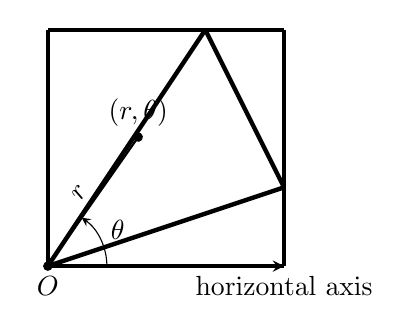
\begin{tikzpicture}
  \draw[thick,->] (0,0) node [below] {$O$} -- (3,0) node [below] {horizontal axis} ;
  \filldraw (0,0) circle (1.5pt);
  \filldraw [rotate=55] (2,0) circle (1.5pt);
  \draw [thick,rotate=55] (0,0)-- node [rotate=55,pos=.5,above] {$r$} (2,0) node [above] {$(r,\theta)$};
  \draw [->] (.75,0) arc(0:55:.75); 
  \draw [rotate=27.5] (1,0) node {$\theta$};


  \draw [ultra thick] (0,0) -- (0,3);
  \draw [ultra thick] (0,0) -- (3,0);
  \draw [ultra thick] (3,0) -- (3,3);
  \draw [ultra thick] (0,3) -- (3,3);

  \draw [ultra thick] (0,0) -- (3,1);
  \draw [ultra thick] (3,1) -- (2,3);
  \draw [ultra thick] (0,0) -- (2,3);



    \end{tikzpicture}
  \end{image}






















\end{document}
